\newpage
\section{Versuchsaufbau}

    \subsection{Szenario}

    Im ersten Schritt wurde das Netzwerk mithilfe von Subnetting getrennt und anschließend unter Verwendung von managebaren NETGEAR-Switches
    in unterschiedliche VLANs unterteilt.

    \subsection{Durchführung}

        \subsubsection{Funktionsprüfung des Netzwerks}
        \begin{table}[H]
            \centering
            \begin{tabular}{l|c|l|c|l|c|l|c|l|c|}
            \multicolumn{1}{l}{} & \multicolumn{1}{l}{PC1} & \multicolumn{1}{l}{PC2} & \multicolumn{1}{l}{PC3} & \multicolumn{1}{l}{PC4}  \\ 
            \cline{2-5}
            PC1&&X&& \\ 
            \cline{2-5}
            PC2&X&&& \\
            \cline{2-5}
            PC3&&&&X \\
            \cline{2-5}
            PC4&&&X& \\
            \cline{2-5}
            \end{tabular}
            \caption{Ergebnistabelle\\ (Erreichbarkeit der einzelnen PCs untereinander) mittels "`ping"'-command}
        \end{table}
        
        \subsubsection{Unterteilung in Subnetze}
        Im folgenden Screenshot ist unser Netzwerkplan dokumentiert, welcher als Grundlage für
        den Versuchsaufbau fungiert.
        \begin{figure}[H]
            \centering
            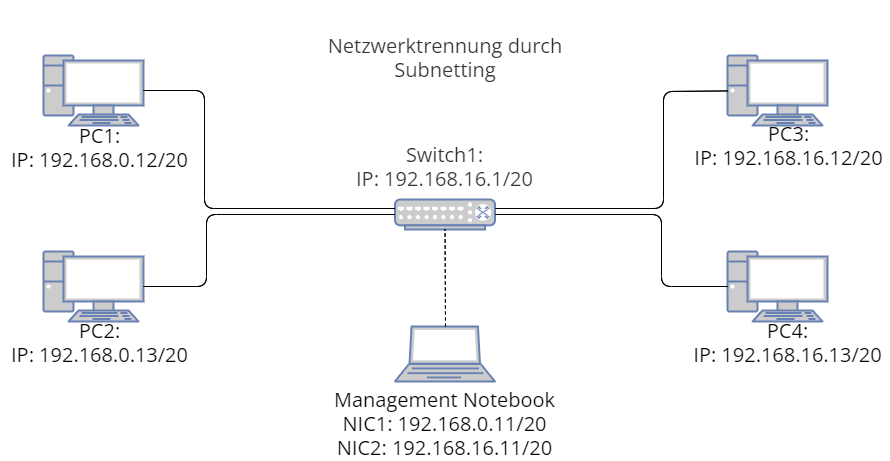
\includegraphics[scale=0.5]{images/Unterteilung in Subnetze/Netzwerkplan_Subnetting_new.png}
            \caption{Netzwerkplan Subnetting}
        \end{figure}
        Die beiden folgenden Screenshots zeigen, dass im Netzwerk zwei PCs erreichbar sind. Im ersten Netzwerk (192.168.0.0) 
        sind die Clients 1 und 2 mit den IP-Adressen 192.168.0.12 und 192.168.0.13 zu finden, während sich im zweiten Netzwerk 
        (192.168.16.0) die Clients 3 und 4 mit den IP-Adressen 192.168.16.12 und 192.168.16.13 befinden. Der Switch(192.168.16.1)
        befindet sich im zeiten Netzwerk(192.168.16.0).
        \begin{figure}[H]
        \centering
            \begin{subfigure}{.5\textwidth}
              \centering
              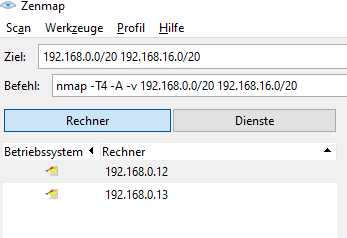
\includegraphics[scale=0.7]{images/Unterteilung in Subnetze/Scan_Subnetz_1.png}
              \caption{Subnetz 1 (192.168.0.0)}
            \end{subfigure}%
            \begin{subfigure}{.5\textwidth}
              \centering
              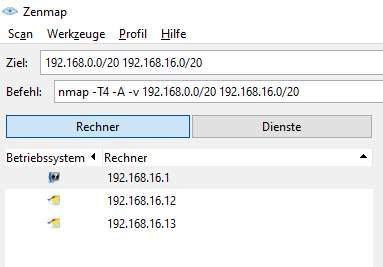
\includegraphics[scale=0.7]{images/Unterteilung in Subnetze/Scan_Subnetz_2.png}
              \caption{Subnetz 2 (192.168.16.0) mit Switch}
            \end{subfigure}
        \caption{Zenmap-Scan Subnetze}
        \end{figure}
        
        Es ist ersichtlich, dass die Clients der beiden Netzwerke nicht miteinander kommunizieren können, wodurch eine abteilungsübergreifende 
        Erreichbarkeit der PCs nicht mehr möglich ist. Dies ist auch in den beiden folgenden Screenshots deutlich erkennbar, 
        in denen der Befehl "`ipconfig"' und "`ping"' in der Befehlszeile des jeweiligen Clients ausgeführt wurde.
        
        \begin{figure}[H]
        \centering
            \begin{subfigure}{\textwidth}
                \centering
                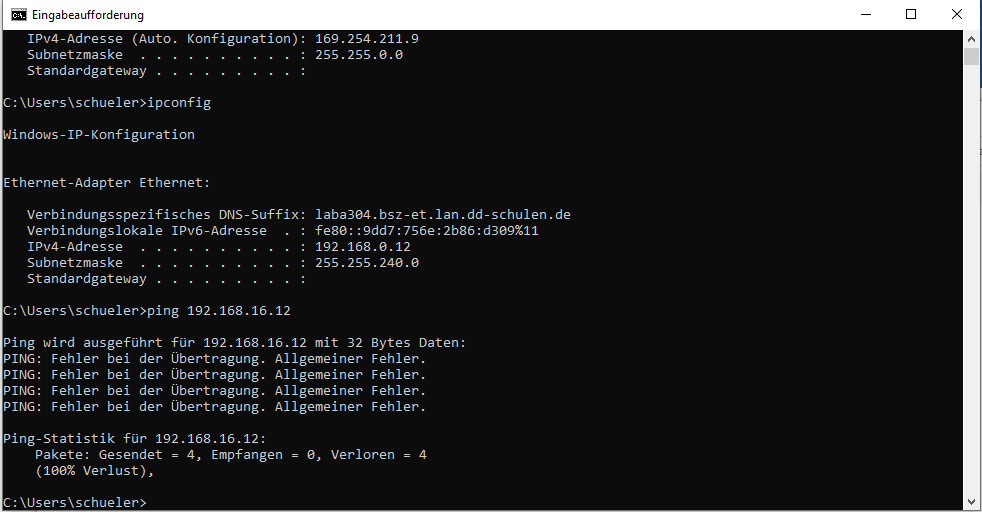
\includegraphics[scale=0.5]{images/Unterteilung in Subnetze/SubnetzPC1_PingPC3.png}
                \caption{ping PC1 zu PC3}
            \end{subfigure}
            \begin{subfigure}{\textwidth}
                \centering
                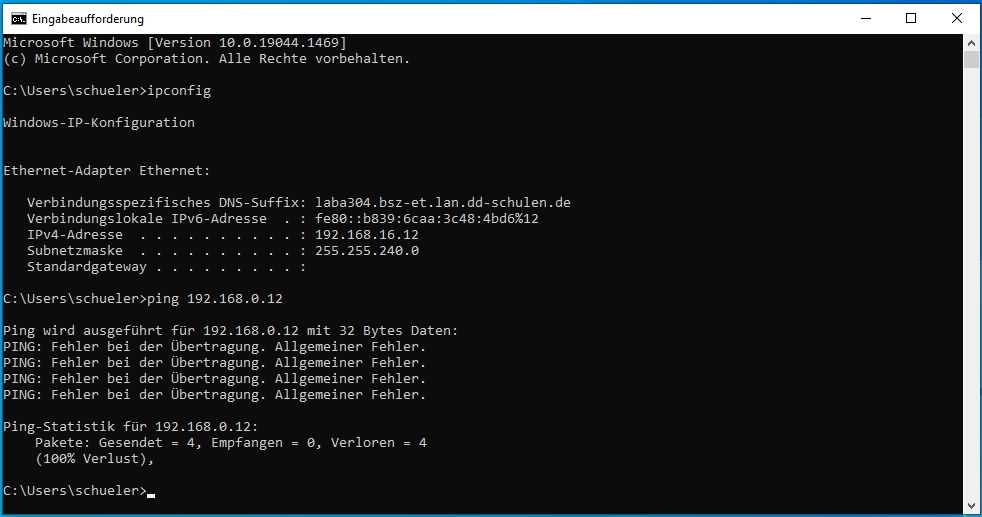
\includegraphics[scale=0.5]{images/Unterteilung in Subnetze/SubnetzPC3_PingPC1.png}
                \caption{ping PC3 zu PC1}
            \end{subfigure}
        \caption{Erreichbarkeit Netzwerke Subnetting}
        \end{figure}

        \newpage
        \subsubsection{Trennung durch VLAN herstellen}
        Im folgenden Screenshot ist unser Netzwerkplan dokumentiert, welcher als Grundlage für
        den Versuchsaufbau der Netzwertrennung durch VLANs fungiert.
        \begin{figure}[H]
            \centering
            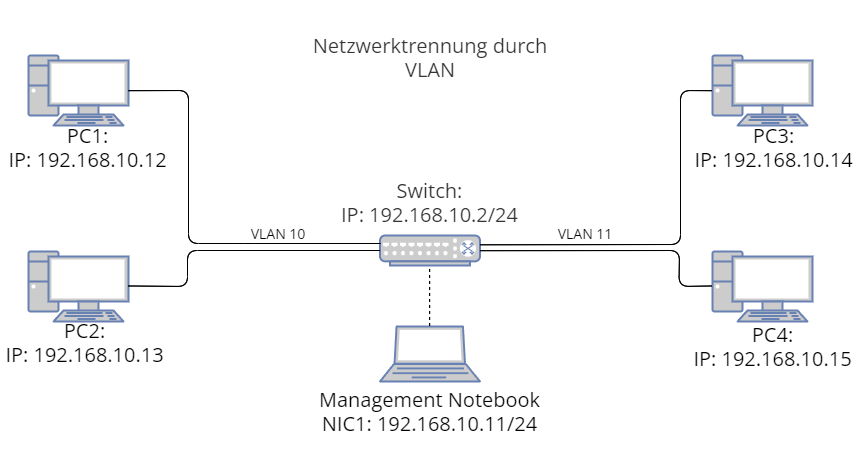
\includegraphics[width=\linewidth]{images/Trennung durch VLAN herstellen/Netzwerkplan_VLAN._portbasiert.png}
            \caption{Netzwerkplan portbasiertes VLAN}
        \end{figure}
        Um die Trennung durch VLANs zu realisieren haben wir als erstes ein portbasiertes VLAN eingerichtet, welches wir
        in den weiteren Aufgaben auf PVID erweitert haben.
        \begin{figure}[H]
        \centering
            \begin{subfigure}{\linewidth}
                \centering
                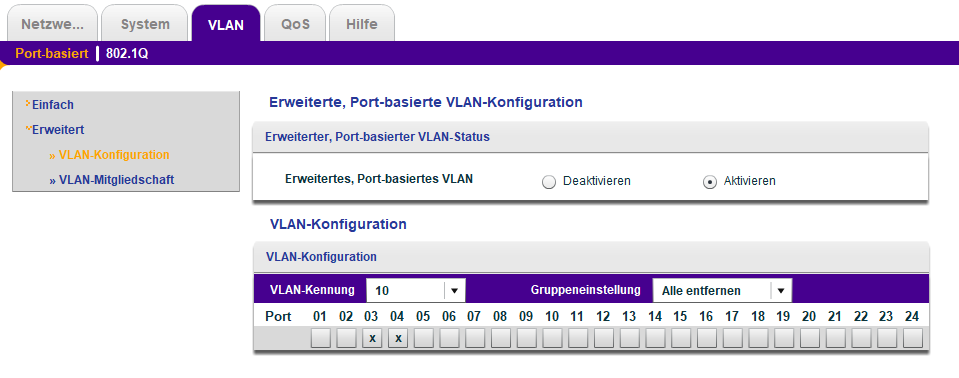
\includegraphics[scale=0.45]{images/Trennung durch VLAN herstellen/VLAN10_Konfiguration.png}
                \caption{VLAN10 Konfiguration}
            \end{subfigure}
            \begin{subfigure}{\linewidth}
                \centering
                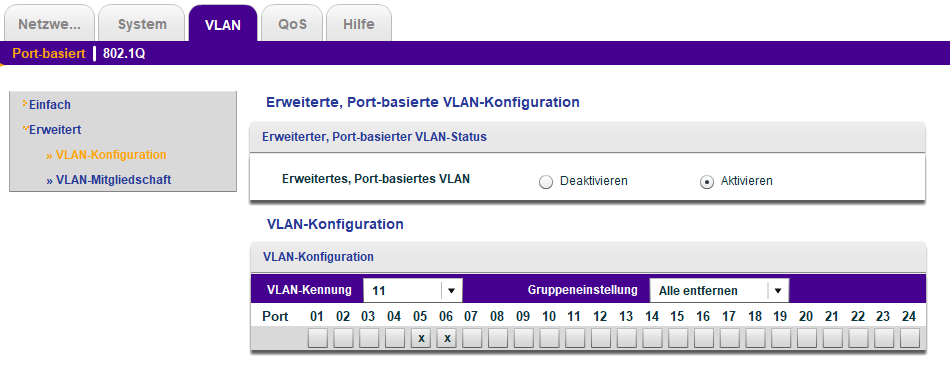
\includegraphics[scale=0.45]{images/Trennung durch VLAN herstellen/VLAN11_Konfiguration.png}
                \caption{VLAN11 Konfiguration}
            \end{subfigure}
        \caption{Konfiguration des portbasierten VLANs}
        \end{figure}

        \newpage
        Die Clients sind hierbei in zwei VLANs getrennt, 10 und 11. In den folgenden Screenshots sind Erreichbarkeiten
        der anderen Clients an dem jeweiligen Client dokumentiert.
        \begin{figure}[H]
        \centering
            \begin{subfigure}{.45\linewidth}
                \centering
                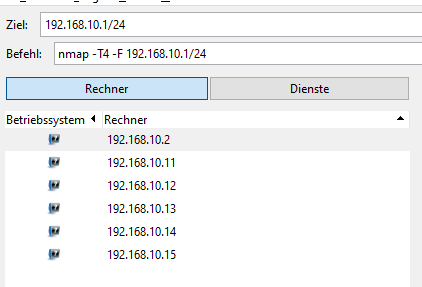
\includegraphics[width=\linewidth]{images/Trennung durch VLAN herstellen/ErreichbarkeitAnliegendAn11.png}
                \caption{Erreichbarkeit anliegend an Management Notebook}
            \end{subfigure}
            \begin{subfigure}{.45\linewidth}
                \centering
                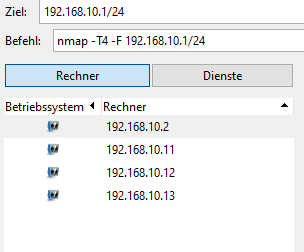
\includegraphics[width=\linewidth]{images/Trennung durch VLAN herstellen/ErreichbarkeitAnliegendAn12.png}
                \caption{Erreichbarkeit anliegend an PC1}
            \end{subfigure}
            \begin{subfigure}{\textwidth}
                \centering
                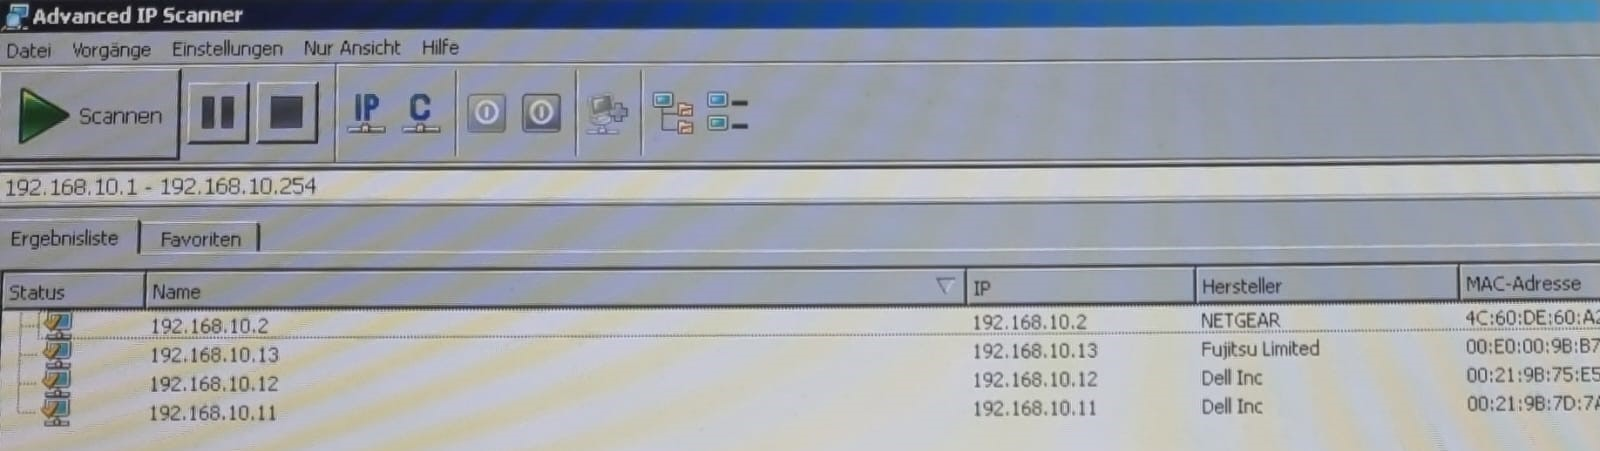
\includegraphics[width=\linewidth]{images/Trennung durch VLAN herstellen/ErreichbarkeitAnliegendAn13.jpg}
                \caption{Erreichbarkeit anliegend an PC2}
            \end{subfigure}
            \begin{subfigure}{\textwidth}
                \centering
                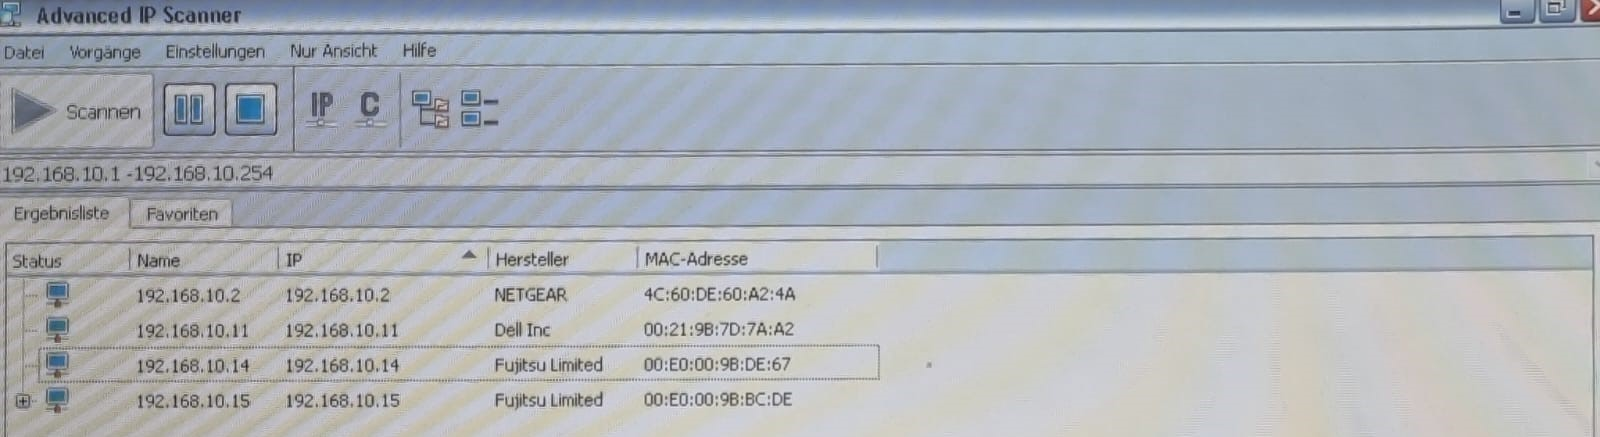
\includegraphics[width=\linewidth]{images/Trennung durch VLAN herstellen/ErreichbarkeitAnliegendAn14.jpg}
                \caption{Erreichbarkeit anliegend an PC3}
            \end{subfigure}
            \begin{subfigure}{\textwidth}
                \centering
                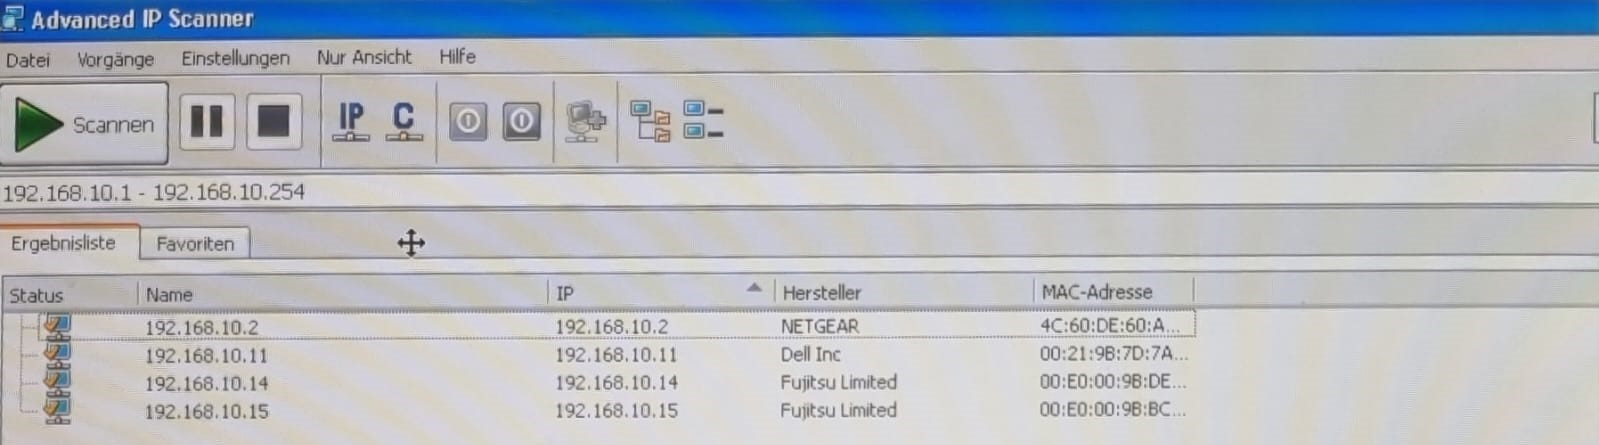
\includegraphics[width=\linewidth]{images/Trennung durch VLAN herstellen/ErreichbarkeitAnliegendAn15.jpg}
                \caption{Erreichbarkeit anliegend an PC4}
            \end{subfigure}
        \caption{Erreichbarkeiten im portbasierten VLAN}
        \end{figure}
        Aus den oben aufgezeigten Screenshots lässt sich erkennen, dass ausschließlich die Clients der 
        zugehörigen VLANs miteinander kommunizieren können.


        \newpage
        \subsubsection{VLAN übergreifenden Server integrieren}
        Um einen VLAN-übergreifenden Server zu integrieren, ist es erforderlich, ein zusätzliches VLAN einzubeziehen, 
        das die Verbindung zwischen den VLANs herstellt, jedoch keine direkte Kommunikation ermöglicht. Im folgenden Netzwerkplan 
        wird mithilfe des Management-Notebooks die Realisierung eines neuen VLANs 12 erreicht, wobei die Mitglieder von VLAN 10 und 11 
        ebenfalls Teil von VLAN 12 sind.
        \begin{figure}[H]
            \centering
            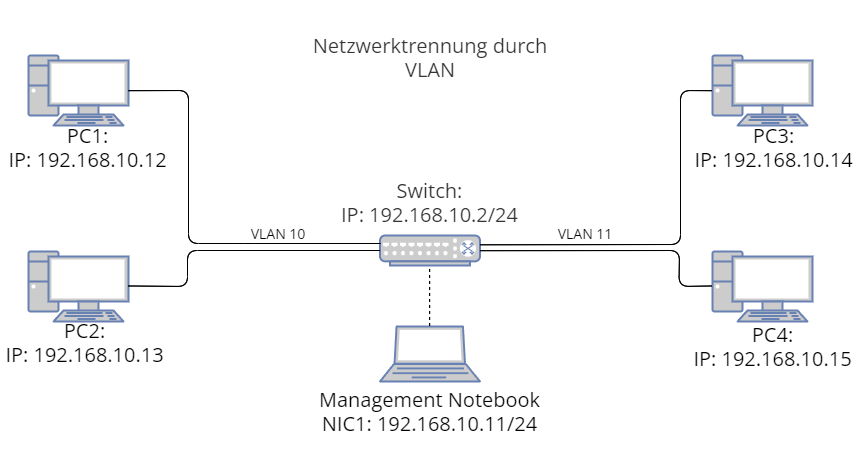
\includegraphics[width=\linewidth]{images/Trennung durch VLAN herstellen/Netzwerkplan_VLAN._portbasiert.png}
            \caption{Netzwerkplan - Integration eines Servers}
        \end{figure}
        Der nächste Screenshot dokumentiert die Konfiguration des Switches zur Einrichtung des VLAN 12.
        Hierbei haben wir von portbasiertem VLAN auf die erweiterte 802.1Q-VLAN-Konfiguration umgestellt.
        \begin{figure}[H]
            \centering
            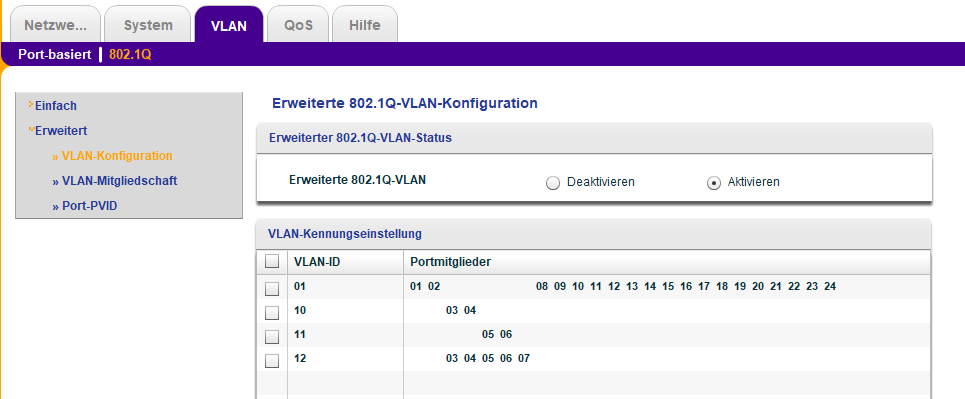
\includegraphics[width=\linewidth]{images/VLAN übergreifenden Server integrieren/VlanKonfigurationMitServer.png}
            \caption{Switch Konfiguration - Integration eines Servers}
        \end{figure}
        \begin{figure}[H]
        \centering
            \begin{subfigure}{\linewidth}
                \centering
                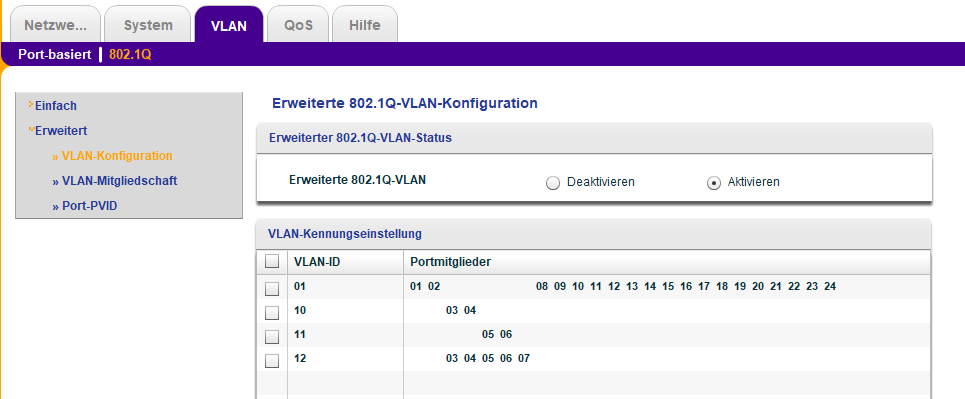
\includegraphics[width=\linewidth]{images/VLAN übergreifenden Server integrieren/VlanKonfigurationMitServer.png}
                \caption{Übersicht der VLAN-Mitgliedschaften}
            \end{subfigure}
            \begin{subfigure}{.49\linewidth}
                \centering
                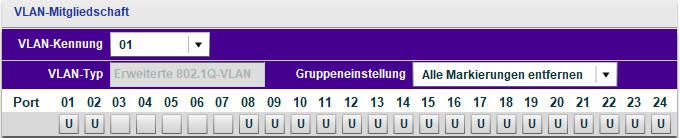
\includegraphics[width=\linewidth]{images/VLAN übergreifenden Server integrieren/VlanMitgliedschaft1.png}
                \caption{VLAN01 - Mitgliedschaften}
            \end{subfigure}
            \begin{subfigure}{.49\linewidth}
                \centering
                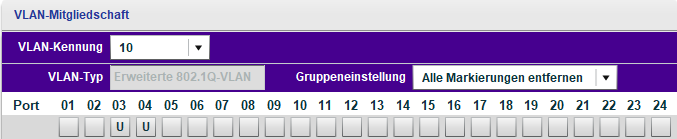
\includegraphics[width=\linewidth]{images/VLAN übergreifenden Server integrieren/VlanMitgliedschaft2.png}
                \caption{VLAN10 - Mitgliedschaften}
            \end{subfigure}
            \begin{subfigure}{.49\linewidth}
                \centering
                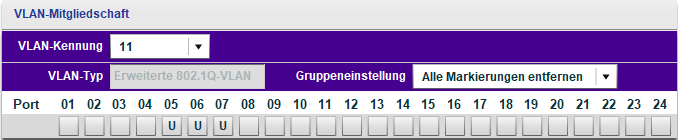
\includegraphics[width=\linewidth]{images/VLAN übergreifenden Server integrieren/VlanMitgliedschaft3.png}
                \caption{VLAN11 - Mitgliedschaften}
            \end{subfigure}
            \begin{subfigure}{.49\linewidth}
                \centering
                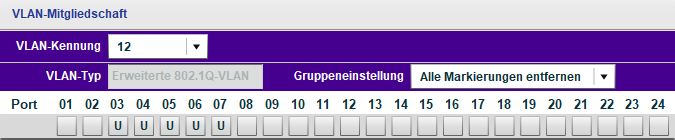
\includegraphics[width=\linewidth]{images/VLAN übergreifenden Server integrieren/VlanMitgliedschaft4.png}
                \caption{VLAN12 - Mitgliedschaften}
            \end{subfigure}
        \caption{Switch Konfiguration - Integration eines Servers}
        \end{figure}
        \begin{figure}[H]
            \centering
            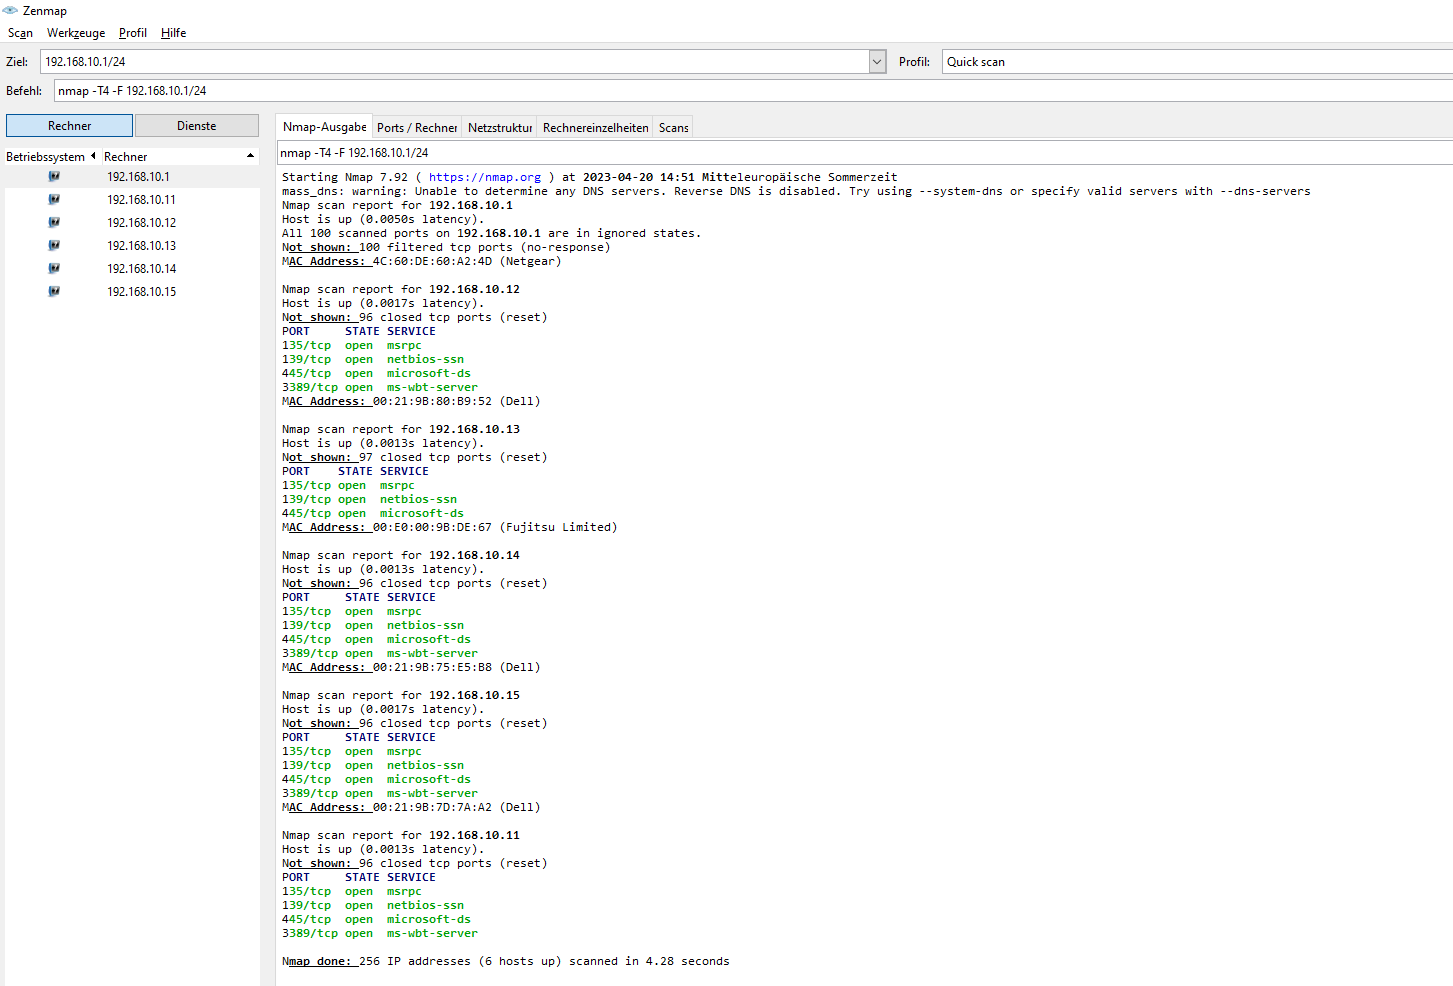
\includegraphics[width=\linewidth]{images/VLAN übergreifenden Server integrieren/serverVLAN12_IP11.png}
            \caption{Zenmap-Scan Server - Integration eines Servers}
        \end{figure}

        \newpage
        \subsubsection{Einrichtung Layer2-Switche}
        Da wir sowohl einen weiteren Switch als auch neue Clients zur Integration der neuen Abteilung benötigten, 
        mussten wir zunächst einen neuen Netzwerkplan erstellen, in welchem die Verbindung mit einem Layer2-Switch ermöglicht wird.
        Hierbei haben wir den zweiten Switch mittels eines Trunking-Ports nach dem Switch-Stacking Verfahren an den ersten Switch angebunden.
        \begin{figure}[H]
            \centering
            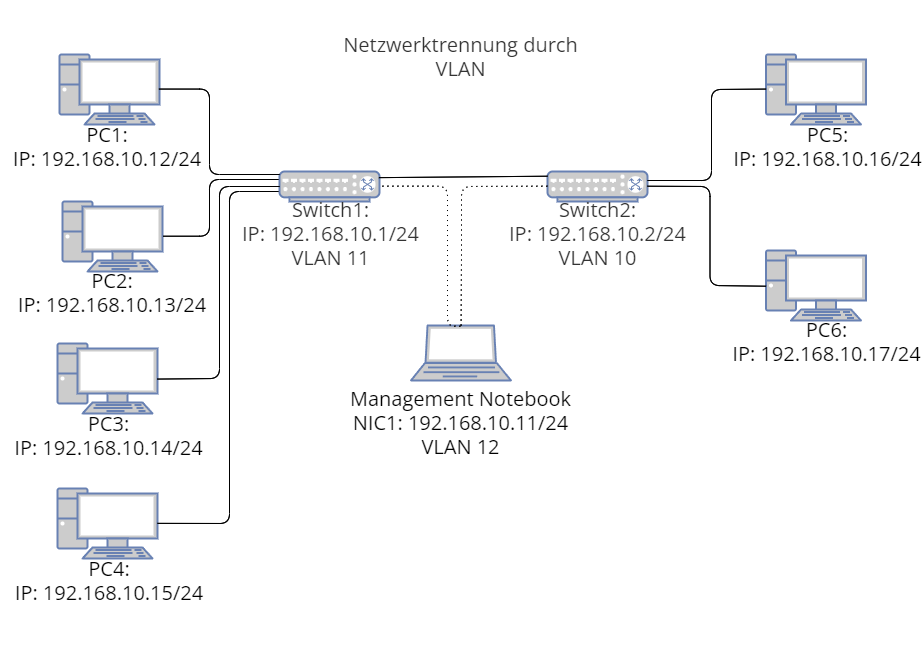
\includegraphics[width=\linewidth]{images/Einrichtung Layer2-Switche/Netzwerkplan_VLAN_switch_stacking.png}
            \caption{Netzwerkplan - Layer2-Switche}
        \end{figure}
        Unser Versuchsaufbau mit dem hinzugefügten Switch, der über Port1 mit dem ersten Switch verbunden ist, sah wie folgt aus:
        \begin{figure}[H]
            \centering
            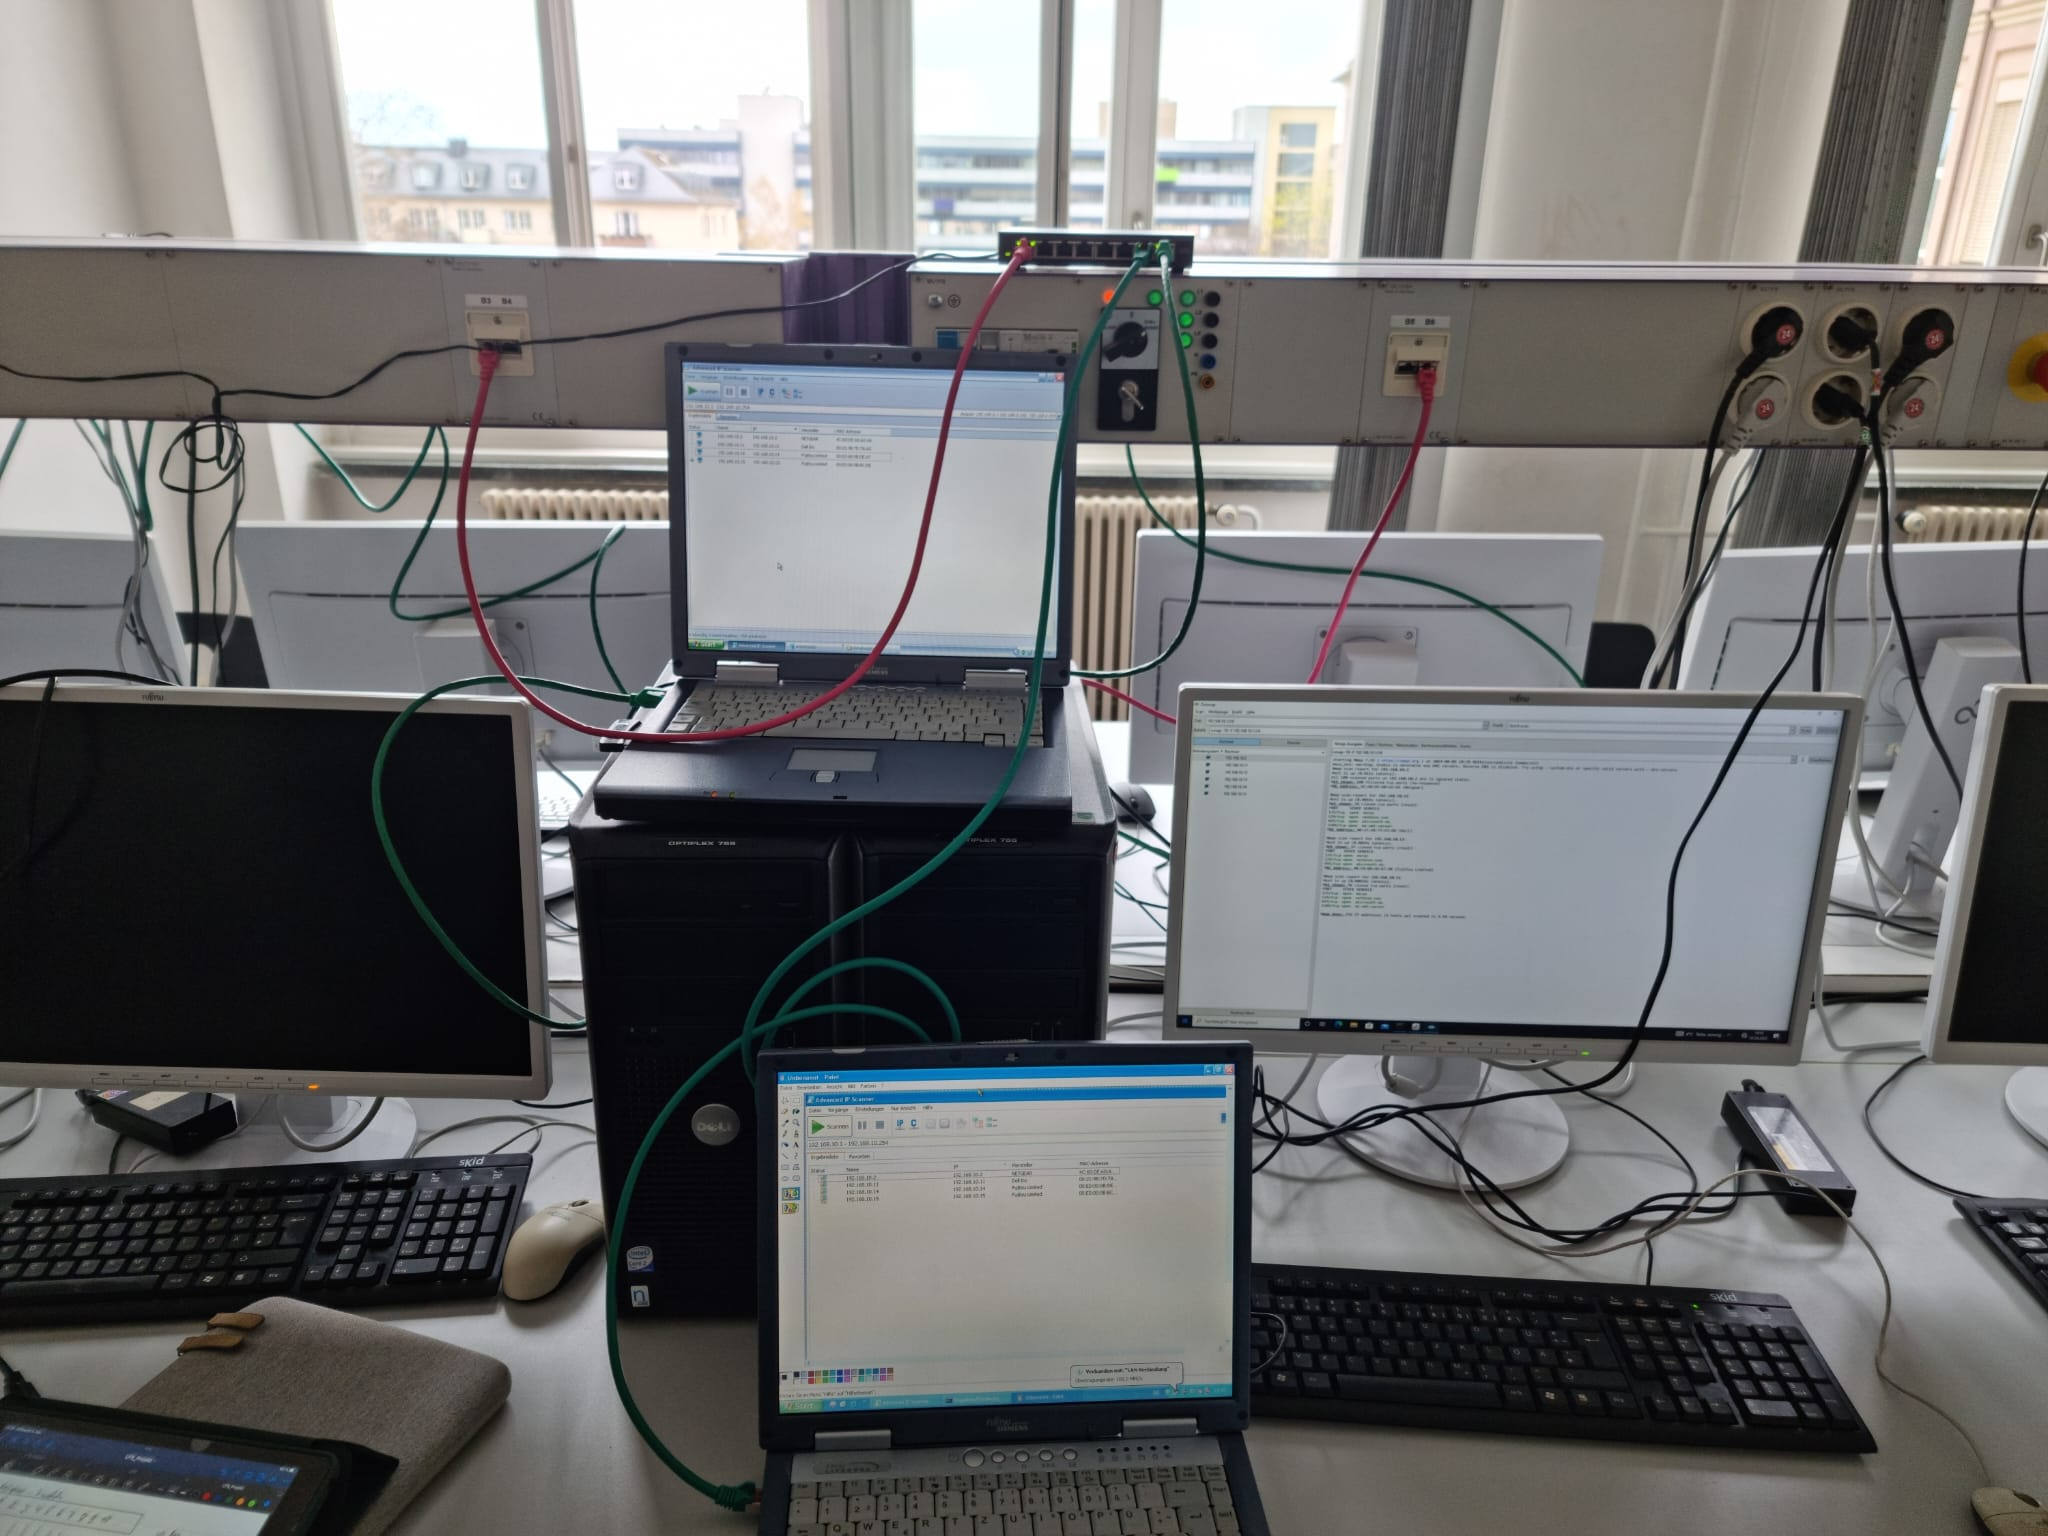
\includegraphics[width=0.6\linewidth]{images/Einrichtung Layer2-Switche/AufbauVersuch.jpg}
            \caption{Versuchsaufbau - Layer2-Switche}
        \end{figure}
        Des weiteren mussten wir die Konfiguration der Switche verändern:
        \begin{figure}[H]
        \centering
            \begin{subfigure}{.49\linewidth}
                \centering
                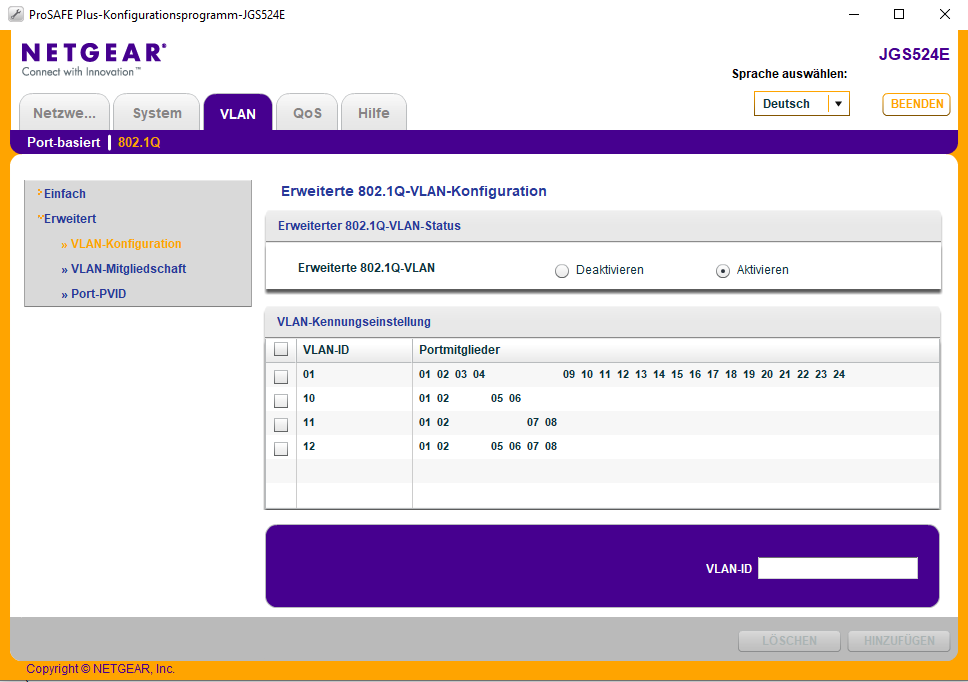
\includegraphics[width=\linewidth]{images/Einrichtung Layer2-Switche/Config_Switch1.png}
                \caption{Mitgliedschaften Switch1}
            \end{subfigure}
            \begin{subfigure}{.49\linewidth}
                \centering
                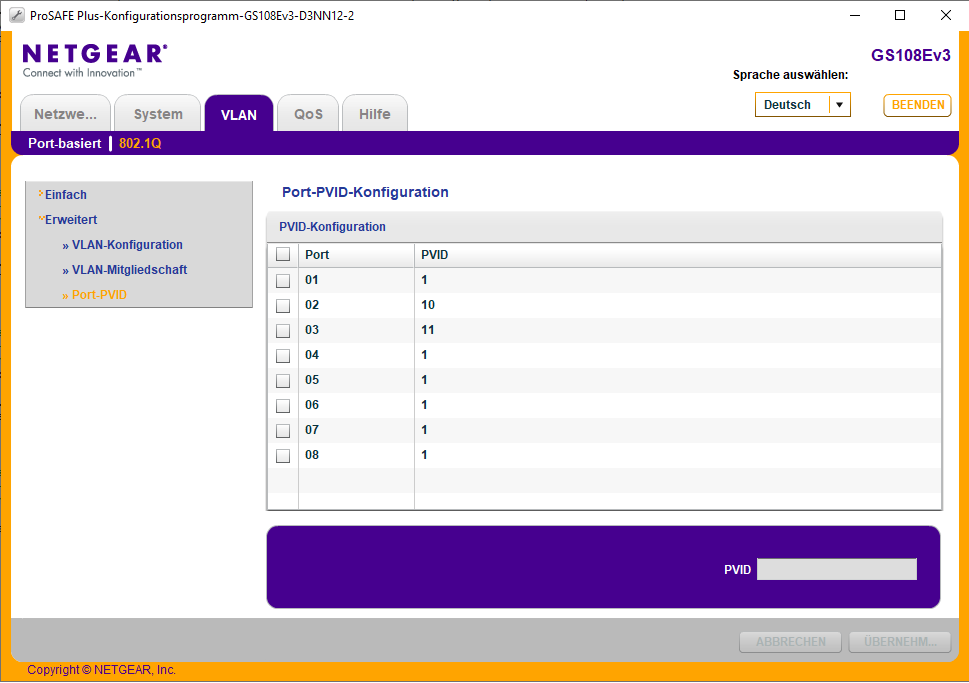
\includegraphics[width=\linewidth]{images/Einrichtung Layer2-Switche/Config_PortPVID_Switch2.png}
                \caption{PVID Switch1}
            \end{subfigure}
            \begin{subfigure}{.49\linewidth}
                \centering
                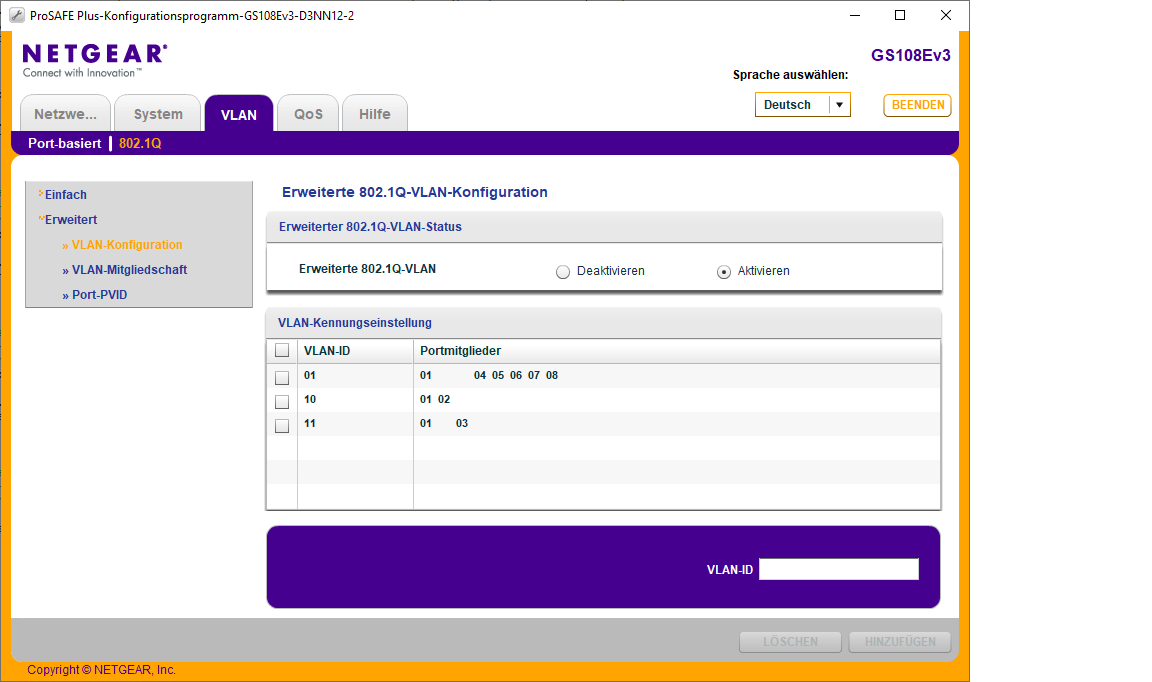
\includegraphics[width=\linewidth]{images/Einrichtung Layer2-Switche/Config_Switch2.png}
                \caption{Mitgliedschaften Switch2}
            \end{subfigure}
            \begin{subfigure}{.49\linewidth}
                \centering
                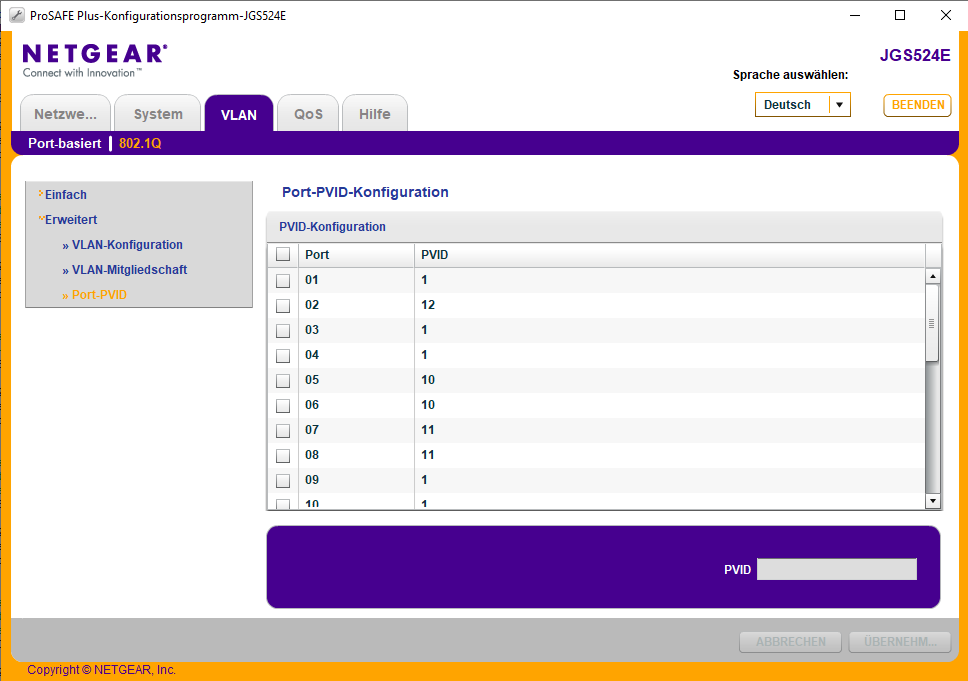
\includegraphics[width=\linewidth]{images/Einrichtung Layer2-Switche/Config_PVID_Switch1.png}
                \caption{PVID Switch2}
            \end{subfigure}
        \caption{Switch Konfiguration - Layer2-Switche}
        \end{figure}
         
        Um eine Kommunikation innerhalb der VLANs über mehrere Switches hinweg zu 
        ermöglichen, werden auf beiden Switches auf Port 1 Datenpakete mit 
        VLAN-Informationen verschickt, die als getaggte Pakete bezeichnet werden.
        Nach folgendem Schema habe wir die Portkonfiguration der Switche durchgeführt, 
        "`T"' steht in diesem Fall für "`Tagged"' und "`U"' für "`Untagged"'.
        \begin{figure}[H]
            \centering
            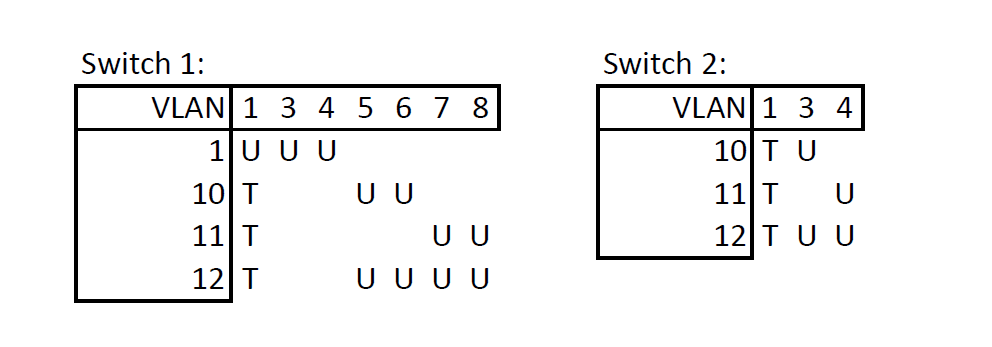
\includegraphics[width=\linewidth]{images/Einrichtung Layer2-Switche/Schema_SwitchKonfiguration_Tagged_untagged.png}
            \caption{Schema Switche - Layer2-Switche}
        \end{figure}
        \newpage
        Im Folgenden wird ersichtlich, dass nur die Clients im jeweiligen VLAN miteinander kommunizieren können:
        \begin{figure}[H]
        \centering
            \begin{subfigure}{\linewidth}
                \centering
                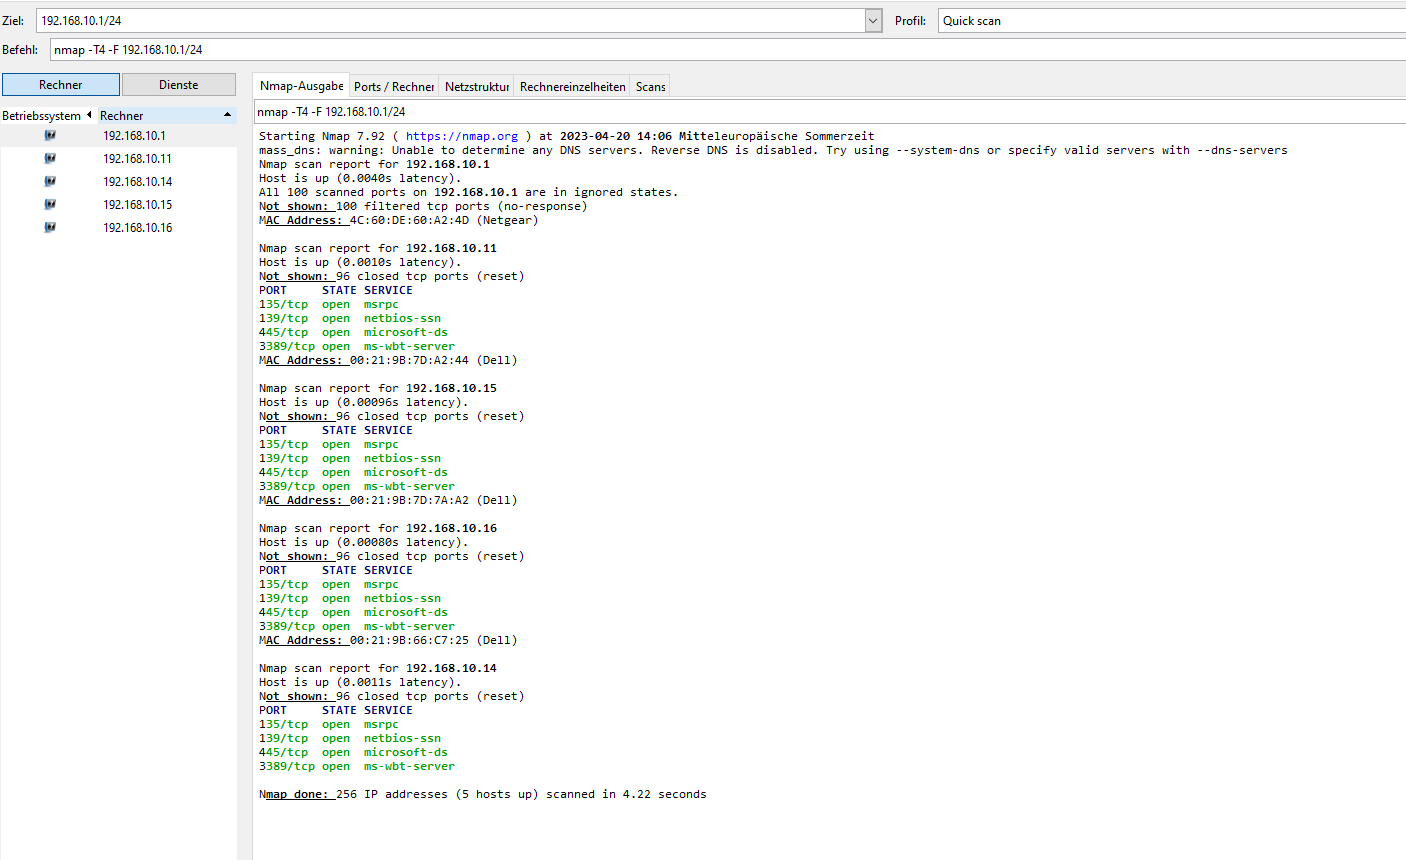
\includegraphics[width=\linewidth]{images/Einrichtung Layer2-Switche/ServerVLAN10Client14.png}
                \caption{Verbindungen Client 14}
            \end{subfigure}
            \begin{subfigure}{\linewidth}
                \centering
                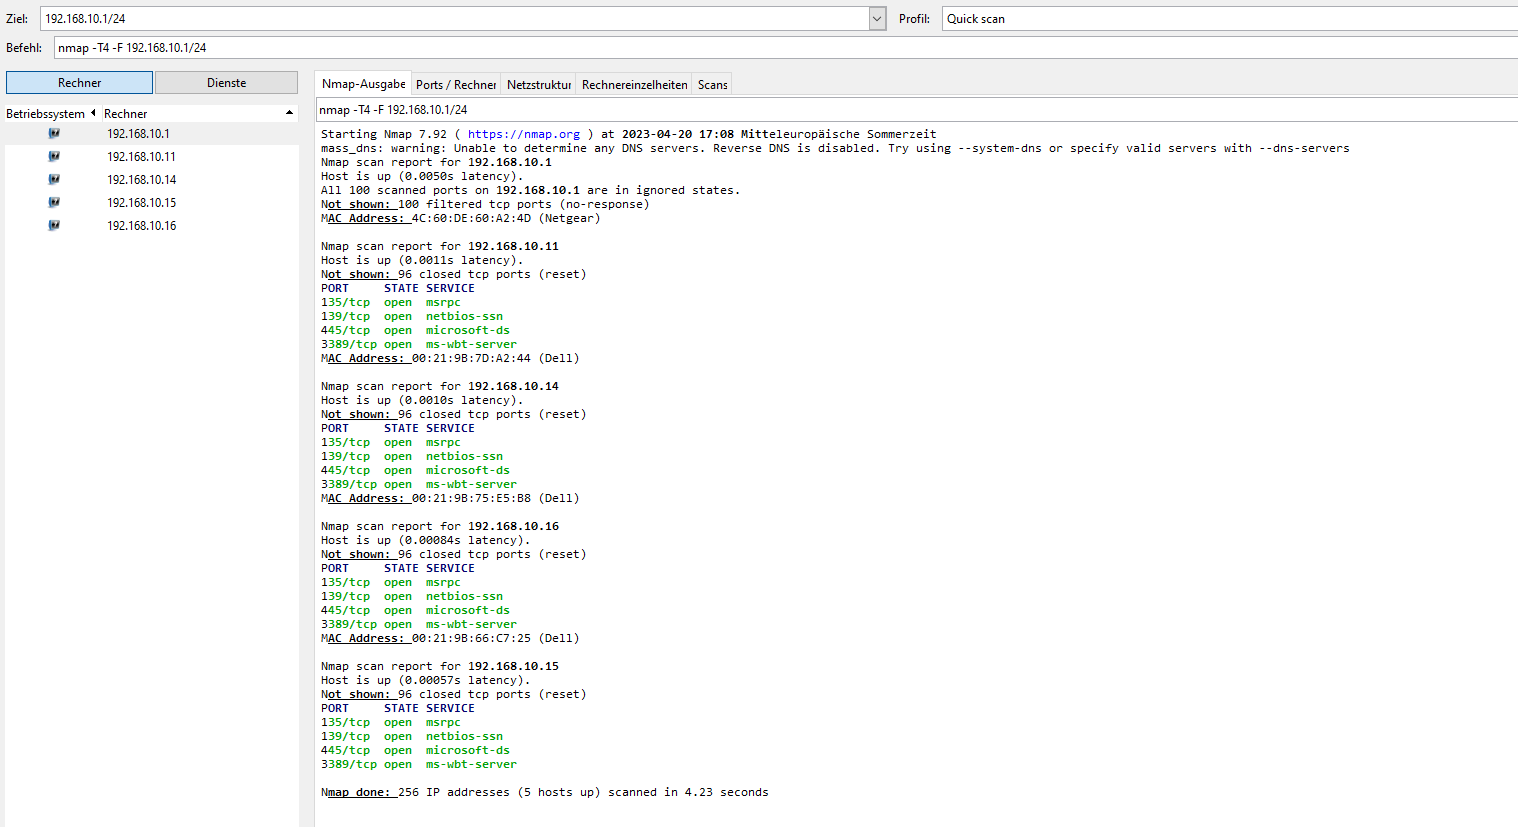
\includegraphics[width=\linewidth]{images/Einrichtung Layer2-Switche/ServerVLAN10Client15.png}
                \caption{Verbindungen Client 15}
            \end{subfigure}
        \caption{Verbindungen VLAN10 - Layer2-Switche}
        \end{figure}%
        \begin{figure}[H]\ContinuedFloat
        \centering
            \begin{subfigure}{\linewidth}
                \centering
                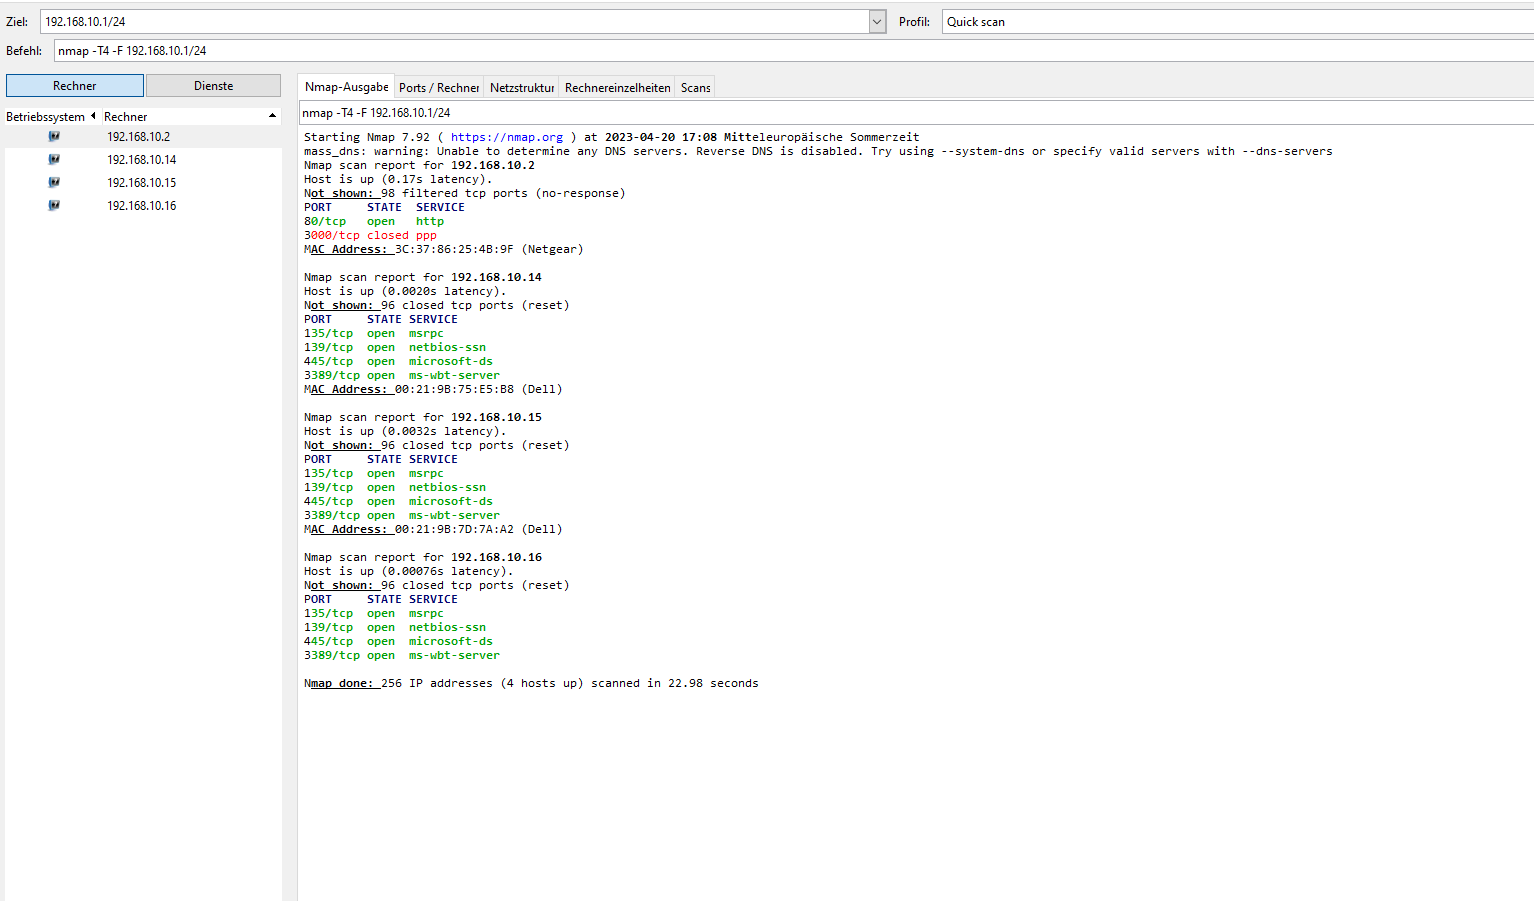
\includegraphics[width=\linewidth]{images/Einrichtung Layer2-Switche/ServerVLAN10Client16.png}
                \caption{Verbindungen Client 16}
            \end{subfigure}
        \caption{Verbindungen VLAN10 - Layer2-Switche}
        \end{figure}
        \begin{figure}[H]
        \centering
            \begin{subfigure}{\linewidth}
                \centering
                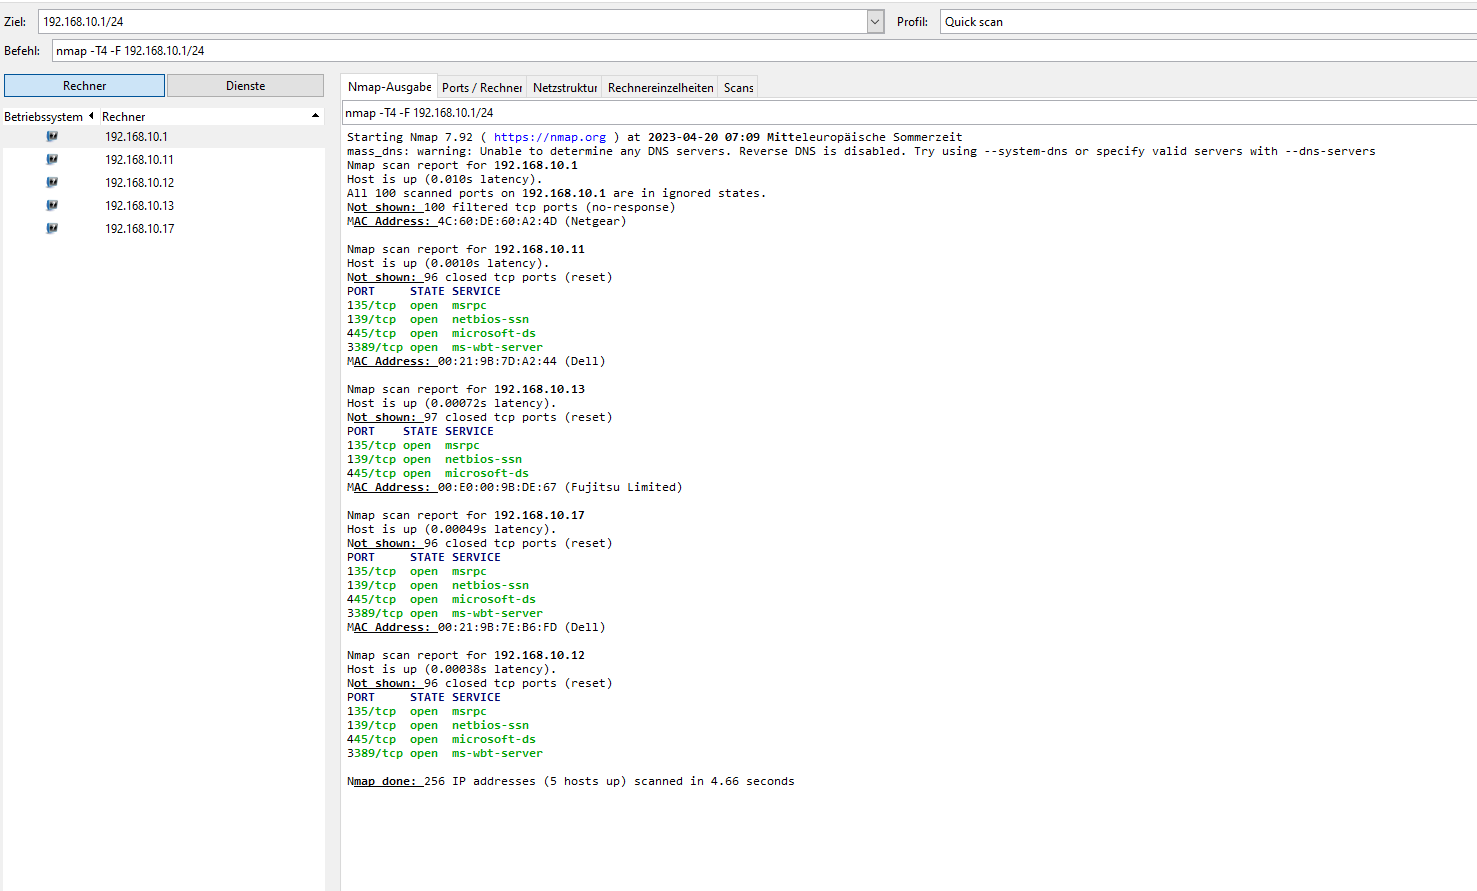
\includegraphics[width=\linewidth]{images/Einrichtung Layer2-Switche/ServerVLAN11Client12.png}
                \caption{Verbindungen Client 12}
            \end{subfigure}
        \caption{Verbindungen VLAN11 - Layer2-Switche}
        \end{figure}%
        \begin{figure}[H]\ContinuedFloat
            \centering
            \begin{subfigure}{\linewidth}
                \centering
                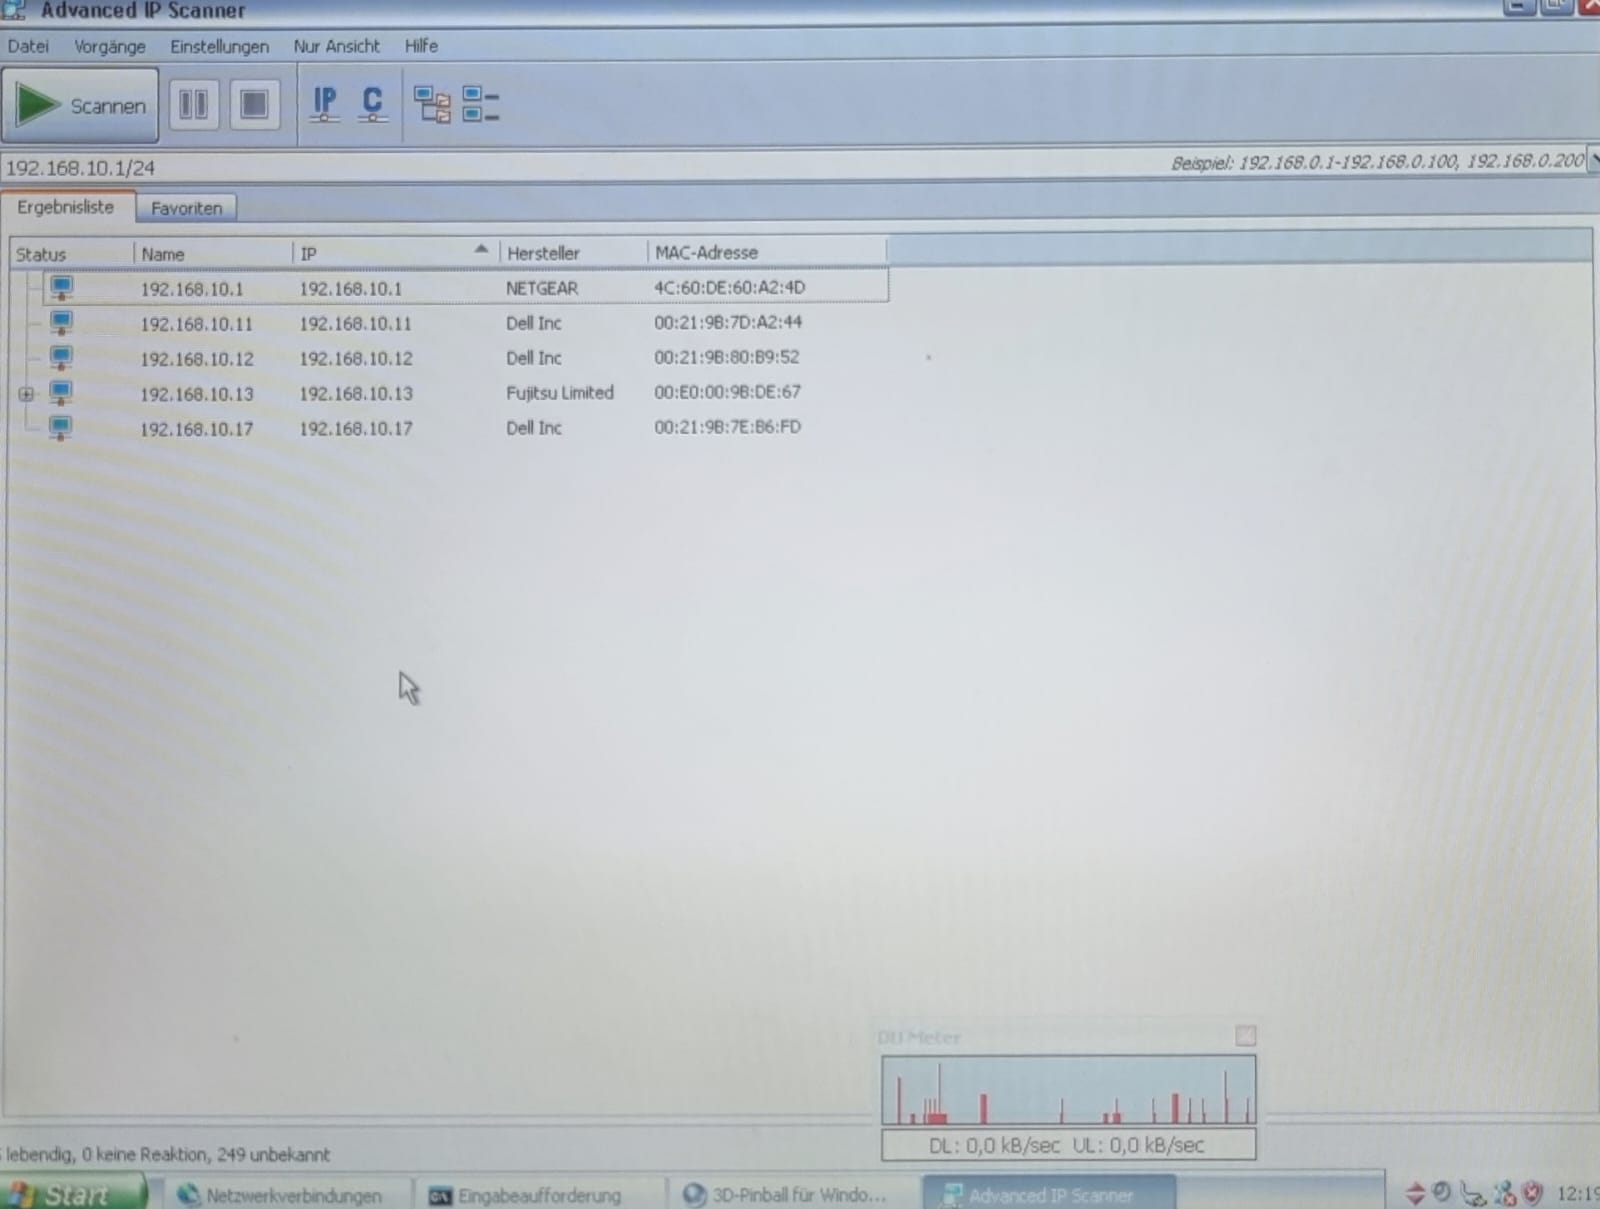
\includegraphics[width=\linewidth]{images/Einrichtung Layer2-Switche/ServerVLAN11Client13.jpg}
                \caption{Verbindungen Client 13}
            \end{subfigure}
            \begin{subfigure}{\linewidth}
                \centering
                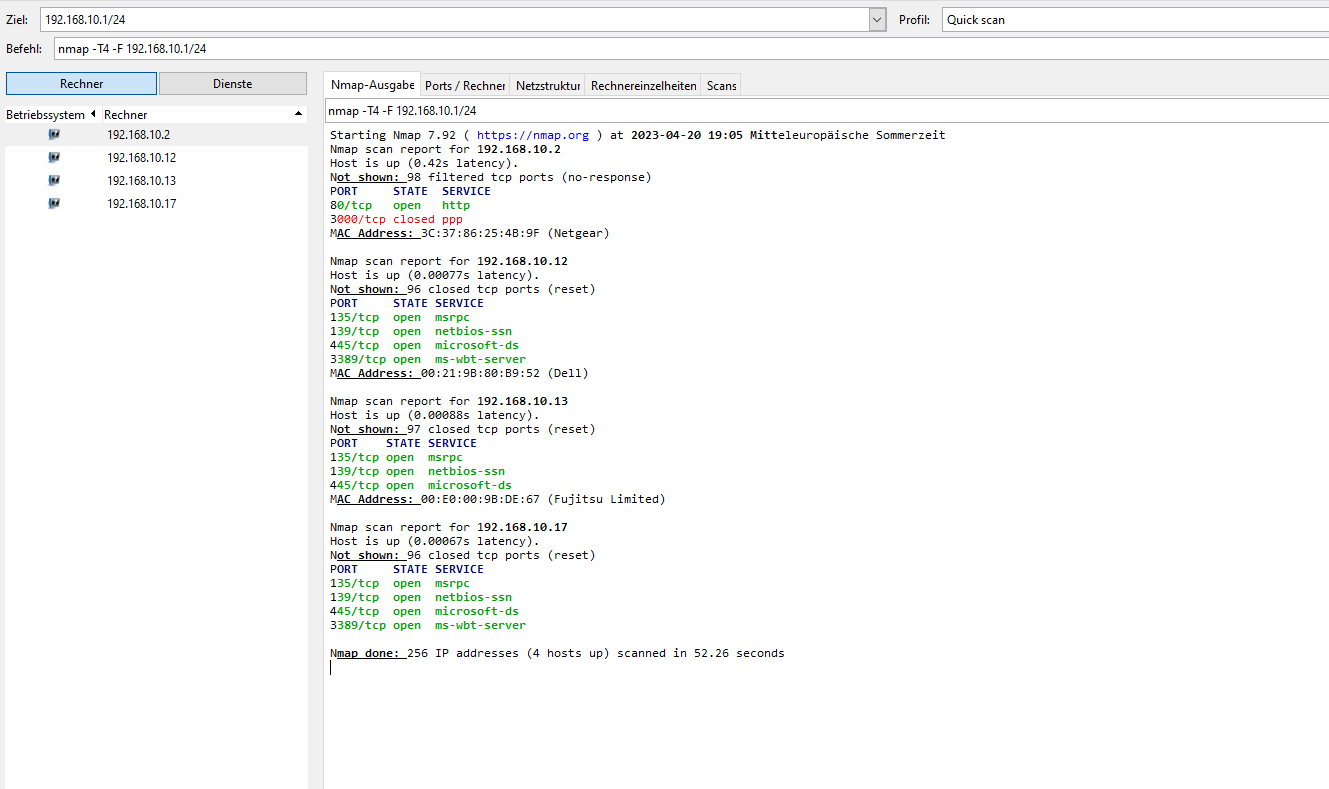
\includegraphics[width=\linewidth]{images/Einrichtung Layer2-Switche/ServerVLAN11Client17.png}
                \caption{Verbindungen Client 17}
            \end{subfigure}
        \caption{Verbindungen VLAN11 - Layer2-Switche}
        \end{figure}



